\documentclass[../Main.tex]{subfiles}

\begin{document}

\section{Visualización}
Con el objetivo de obtener una primera impresión de los datos, se procedió a graficar y tabular estos en bruto y buscar correlaciones superficiales entre los datos. De los sets de datos entregados, algunos se pueden visualizar:
\newline \par

\textbf{POWER: Consumo energético, variable a predecir}
\begin{center}
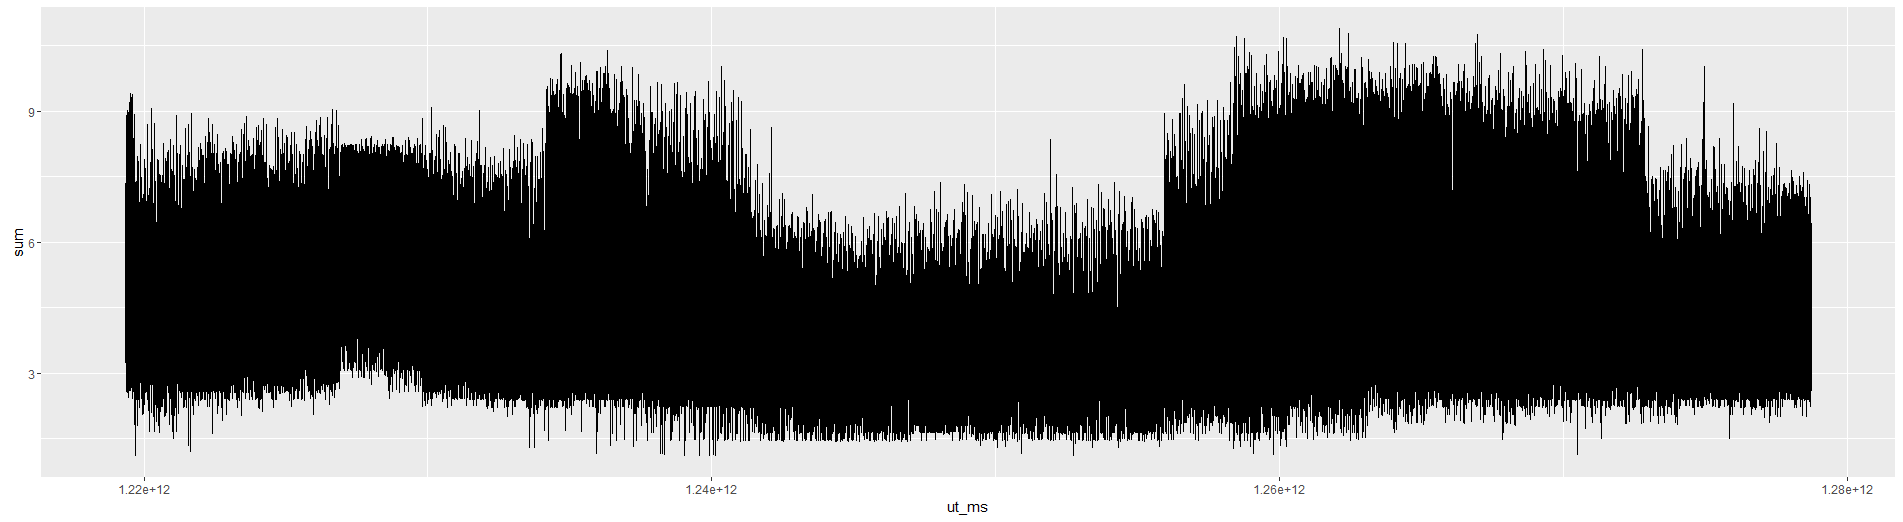
\includegraphics[width=\linewidth, clip]{Assets/powerSum.png}
\textbf{Figura 1.} Suma de potencias para el primer año $power$
\end{center}

\textbf{SAAF: Aspectos solares}
\begin{center}
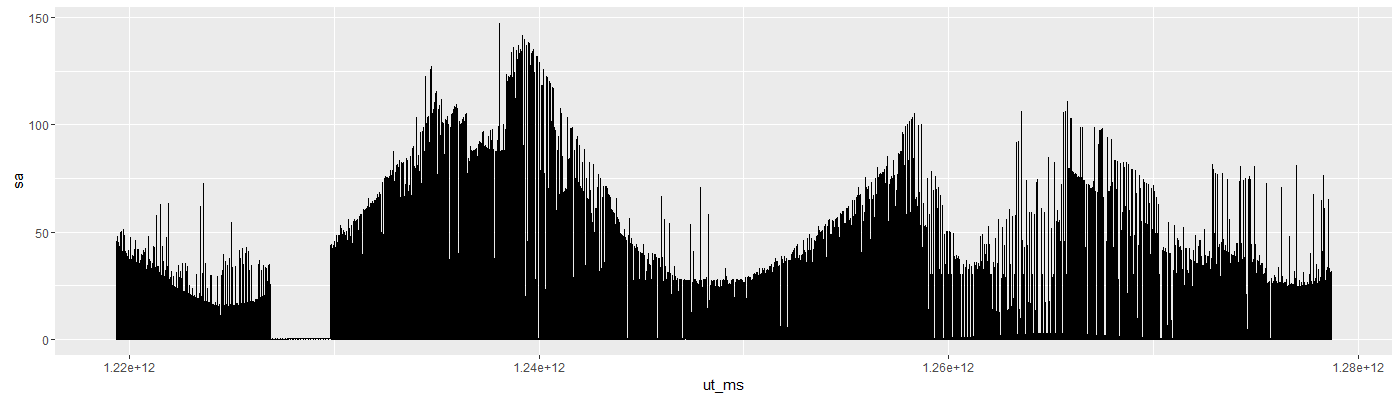
\includegraphics[width=\linewidth, clip]{Assets/saaf1saAll-Stretch.png}
\textbf{Figura 2.} Incidencia Solar para el primer año $saaf\$sa$
\end{center}

\textbf{LTDATA: Información de periodos extendidos}
\begin{center}
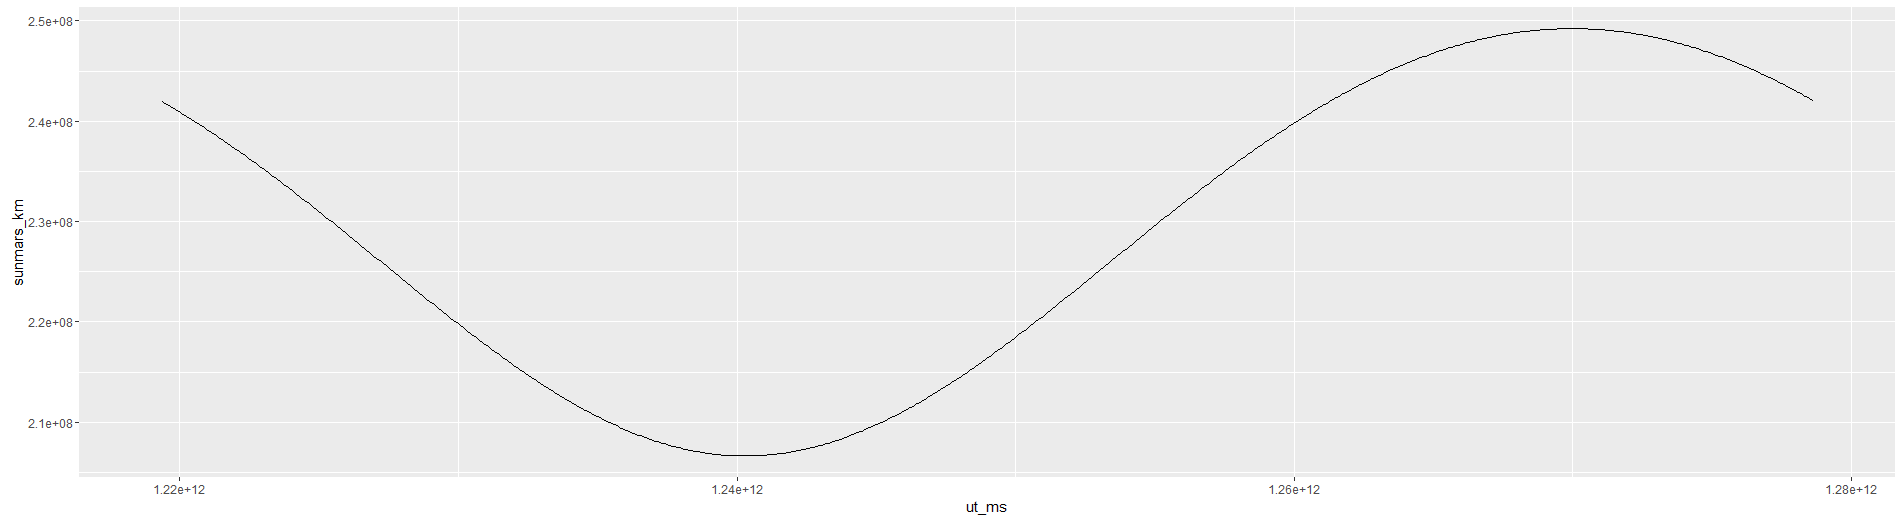
\includegraphics[width=\linewidth, clip]{Assets/sunMars_km.png}
\textbf{Figura 3.} Distancia Sol-Marte para el primer año
\end{center}

Los otros sets del problema tienen datos que no se pueden visualizar de forma directa. Estos están estructurados en el siguiente formato:
\newline \par

\textbf{DMOP: Detalles de la planificación de operación}
\begin{center}
\textbf{Tabla 1.} Muestra registros de dmop.csv\\
\begin{tabular}{|l|l|}\hline
ut\_ms        & subsystem \\ \hline
1219363211000 & AXXX301A  \\
1219364909000 & AAAAF20C1 \\
1219364924000 & AAAAF60A1 \\
1219366035000 & AXXX380A  \\
1219366635000 & ASEQ4200  \\
1219367381000 & ATTTF301E \\ \hline
\end{tabular}
\\[20pt]
\end{center}

\textbf{FTL: Eventos de la trayectoria de la nave}
\begin{center}
\textbf{Tabla 2.} Muestra registros de ftl.csv\\
\begin{tabular}{|l|l|l|l|}\hline
utb\_ms       & ute\_ms       & type  & flagcomms \\ \hline
1219363213000 & 1219365494000 & EARTH & FALSE     \\
1219369619000 & 1219370253000 & SLEW  & FALSE     \\
1219370253000 & 1219373093000 & NADIR & FALSE     \\
1219373093000 & 1219374563000 & SLEW  & FALSE     \\
1219376633000 & 1219381144000 & EARTH & TRUE      \\ \hline
\end{tabular}
\\[20pt]
\end{center}

\textbf{EVTF: Otros eventos}
\begin{center}
\textbf{Tabla 3.} Muestra registros de evtf.csv\\
\begin{tabular}{|l|l|}\hline
ut\_ms        & description                                                                                    \\ \hline
1219365755000 & "NNO\_AOS\_05\_/\_RTLT\_02373"                                                                 \\
1219368640000 & "4000\_KM\_DESCEND"                                                                            \\
1219369280000 & "MRB\_/\_RANGE\_06000KM\_START"                                                                \\
1219369855000 & "OCC\_MARS\_200KM\_START\_/\_RA\_181.68\_/\_OMP\_(296.35  -46.48)\_/\_SZA\_077" \\
1219369949000 & "OCC\_MARS\_START\_/\_RA\_181.69\_/\_DE\_-00.08\_/\_OMP\_(299.32         -43.44)\_/\_SZA\_076" \\ \hline
\end{tabular}
\\[20pt]
\end{center}

Al graficar los valores de potencia, los datos de incidencia solar y los datos de misión, se puede apreciar que existe una ligera correlación entre los anteriores, por lo que se procedió a trabajar sobre estos datos en primera instancia. 
\end{document}